\begin{figure}[tbp]
\centering
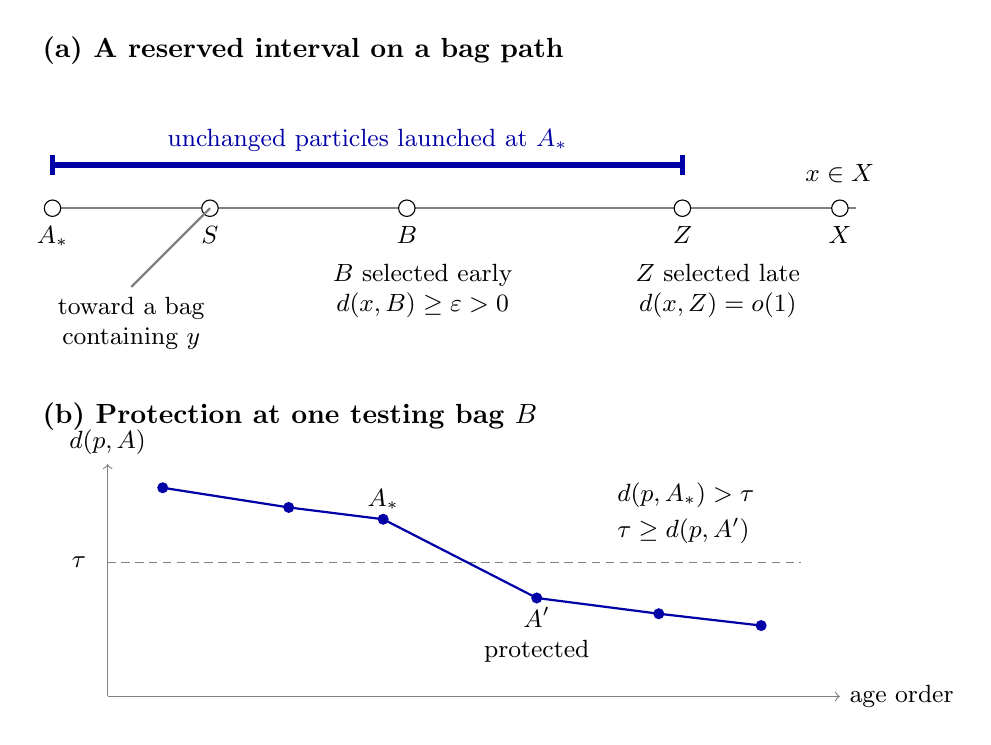
\begin{tikzpicture}[x=1cm,y=1cm,font=\small,
 bag/.style={circle,draw,fill=white,inner sep=2.1pt},
 retained/.style={blue!65!black,line width=2pt}]
 \node[anchor=west,font=\bfseries] at (-.25,2.0) {(a) A reserved interval on a bag path};
 \draw[gray,thick] (0,0)--(10.2,0);
 \foreach \x/\name in {0/A_*,2/S,4.5/B,8/Z,10/X} {
   \node[bag,label=below:$\name$] at (\x,0) {};
 }
 \draw[gray,thick] (2,0)--(1,-1);
 \node[below,align=center] at (1,-1) {toward a bag\\containing $y$};
 \draw[retained] (0,.55)--(8,.55);
 \draw[retained] (0,.42)--(0,.68);
 \draw[retained] (8,.42)--(8,.68);
 \node[blue!65!black,above] at (4,.6) {unchanged particles launched at $A_*$};
 \node[above,align=center] at (4.5,0) {\strut};
 \node[align=center] at (4.7,-1.05) {$B$ selected early\\$d(x,B)\ge\varepsilon>0$};
 \node[align=center] at (8.45,-1.05) {$Z$ selected late\\$d(x,Z)=o(1)$};
 \node[above] at (10,.2) {$x\in X$};
 \node[anchor=west,font=\bfseries] at (-.25,-2.65) {(b) Protection at one testing bag $B$};
 \draw[->,gray] (.7,-6.2)--(10,-6.2) node[right,black] {age order};
 \draw[->,gray] (.7,-6.2)--(.7,-3.25) node[above,black] {$d(p,A)$};
 \draw[gray,densely dashed] (.7,-4.5)--(9.5,-4.5);
 \node[anchor=east] at (.55,-4.5) {$\tau$};
 \draw[blue!65!black,thick] (1.4,-3.55)--(3,-3.8)--(4.2,-3.95)--(6.15,-4.95)--(7.7,-5.15)--(9,-5.3);
 \foreach \x/\y in {1.4/-3.55,3/-3.8,4.2/-3.95,6.15/-4.95,7.7/-5.15,9/-5.3}
  {\fill[blue!65!black] (\x,\y) circle (2pt);}
 \node[above] at (4.2,-3.95) {$A_*$};
 \node[below,align=center] at (6.15,-4.95) {$A'$\\protected};
 \node[anchor=west] at (7.05,-3.65) {$d(p,A_*)>\tau$};
 \node[anchor=west] at (7.05,-4.1) {$\tau\ge d(p,A')$};
\end{tikzpicture}
\caption{The two orders in the anchor argument.
In (a), the selected early bag $B$ and late terminal bag $Z$ lie in the
reservation of $A_*$; the branch toward $y$ makes $B$ a testing bag on
the path to $Z$. The horizontal axis records bag order, not metric
distance, and no first late or last early bag is depicted.
In (b), the entries are ordered by launch time in the list at $B$.
The distance list is nonincreasing. The immediate successor $A'$ is
protected when one of the thresholds $\tau=L/100$ or $\tau=JL$ lies
between its distance and that of $A_*$, where $L=d(p,q)$ is supplied
by Lemma~\ref{lem:anchor-obstruction}. All spacings are schematic.}
\label{fig:anchor-reservations}
\end{figure}
